\section*{Supplementary Information}

\subsection*{Supplementary Figure 1: NDVI-based Contrast Enhancement}

\begin{figure}[h!]
    \centering
    % First image
    \begin{subfigure}[b]{0.48\textwidth} % Adjust width as needed for spacing
        \centering
        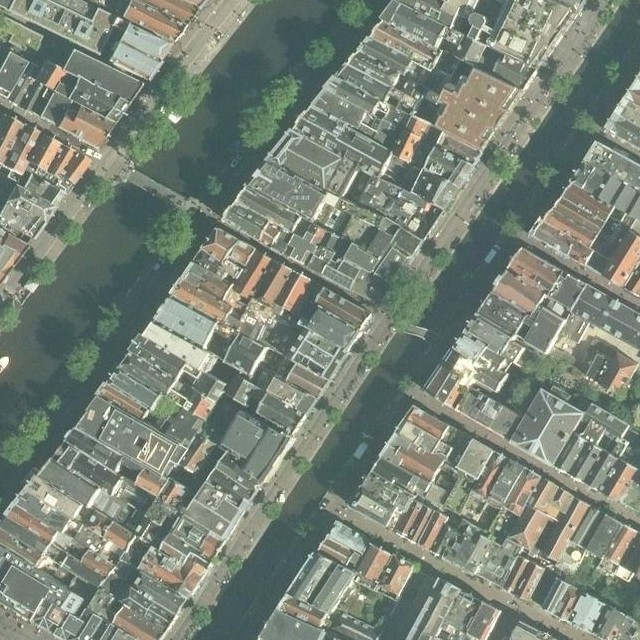
\includegraphics[width=\linewidth, height=\linewidth, keepaspectratio]{figures/methods/RGB_zone0.jpeg}
        \caption{Original Aerial RGB Image}
        \label{fig:supp_ndvi_original}
    \end{subfigure}
    \hfill % Adds horizontal space between subfigures
    % Second image
    \begin{subfigure}[b]{0.48\textwidth}
        \centering
        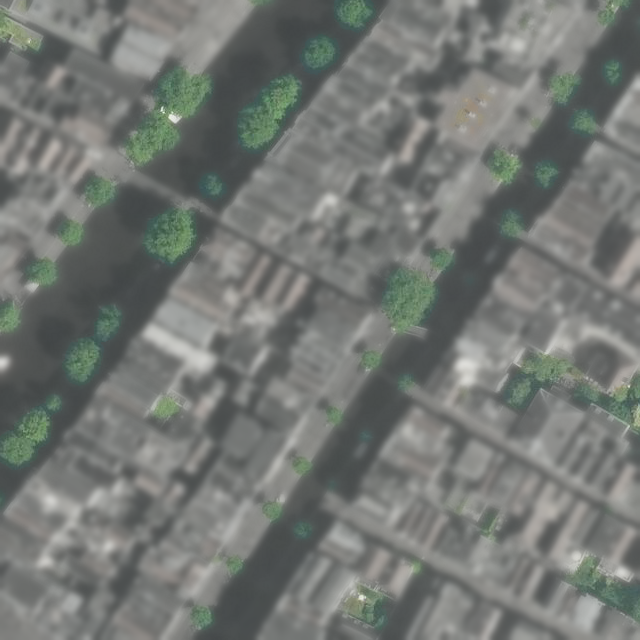
\includegraphics[width=\linewidth, height=\linewidth, keepaspectratio]{figures/methods/06_final_combined.png}
        \caption{NDVI-Enhanced Image}
        \label{fig:supp_ndvi_preprocessed}
    \end{subfigure}
    \caption{\textbf{NDVI-based contrast enhancement workflow.} The preprocessing pipeline applies NDVI-based contrast enhancement to aerial RGB imagery to improve detection and segmentation of individual urban trees. (a) Original aerial RGB image showing urban tree canopies. (b) NDVI-enhanced image with improved contrast for tree crown delineation. This preprocessing step significantly improves the performance of deep learning segmentation models by emphasizing vegetation features while suppressing background urban surfaces.}
    \label{fig:supp_ndvi_enhancement}
\end{figure}

\subsection*{Supplementary Figure 2: Tree Species Distribution}

\begin{figure}[h!]
    \centering
    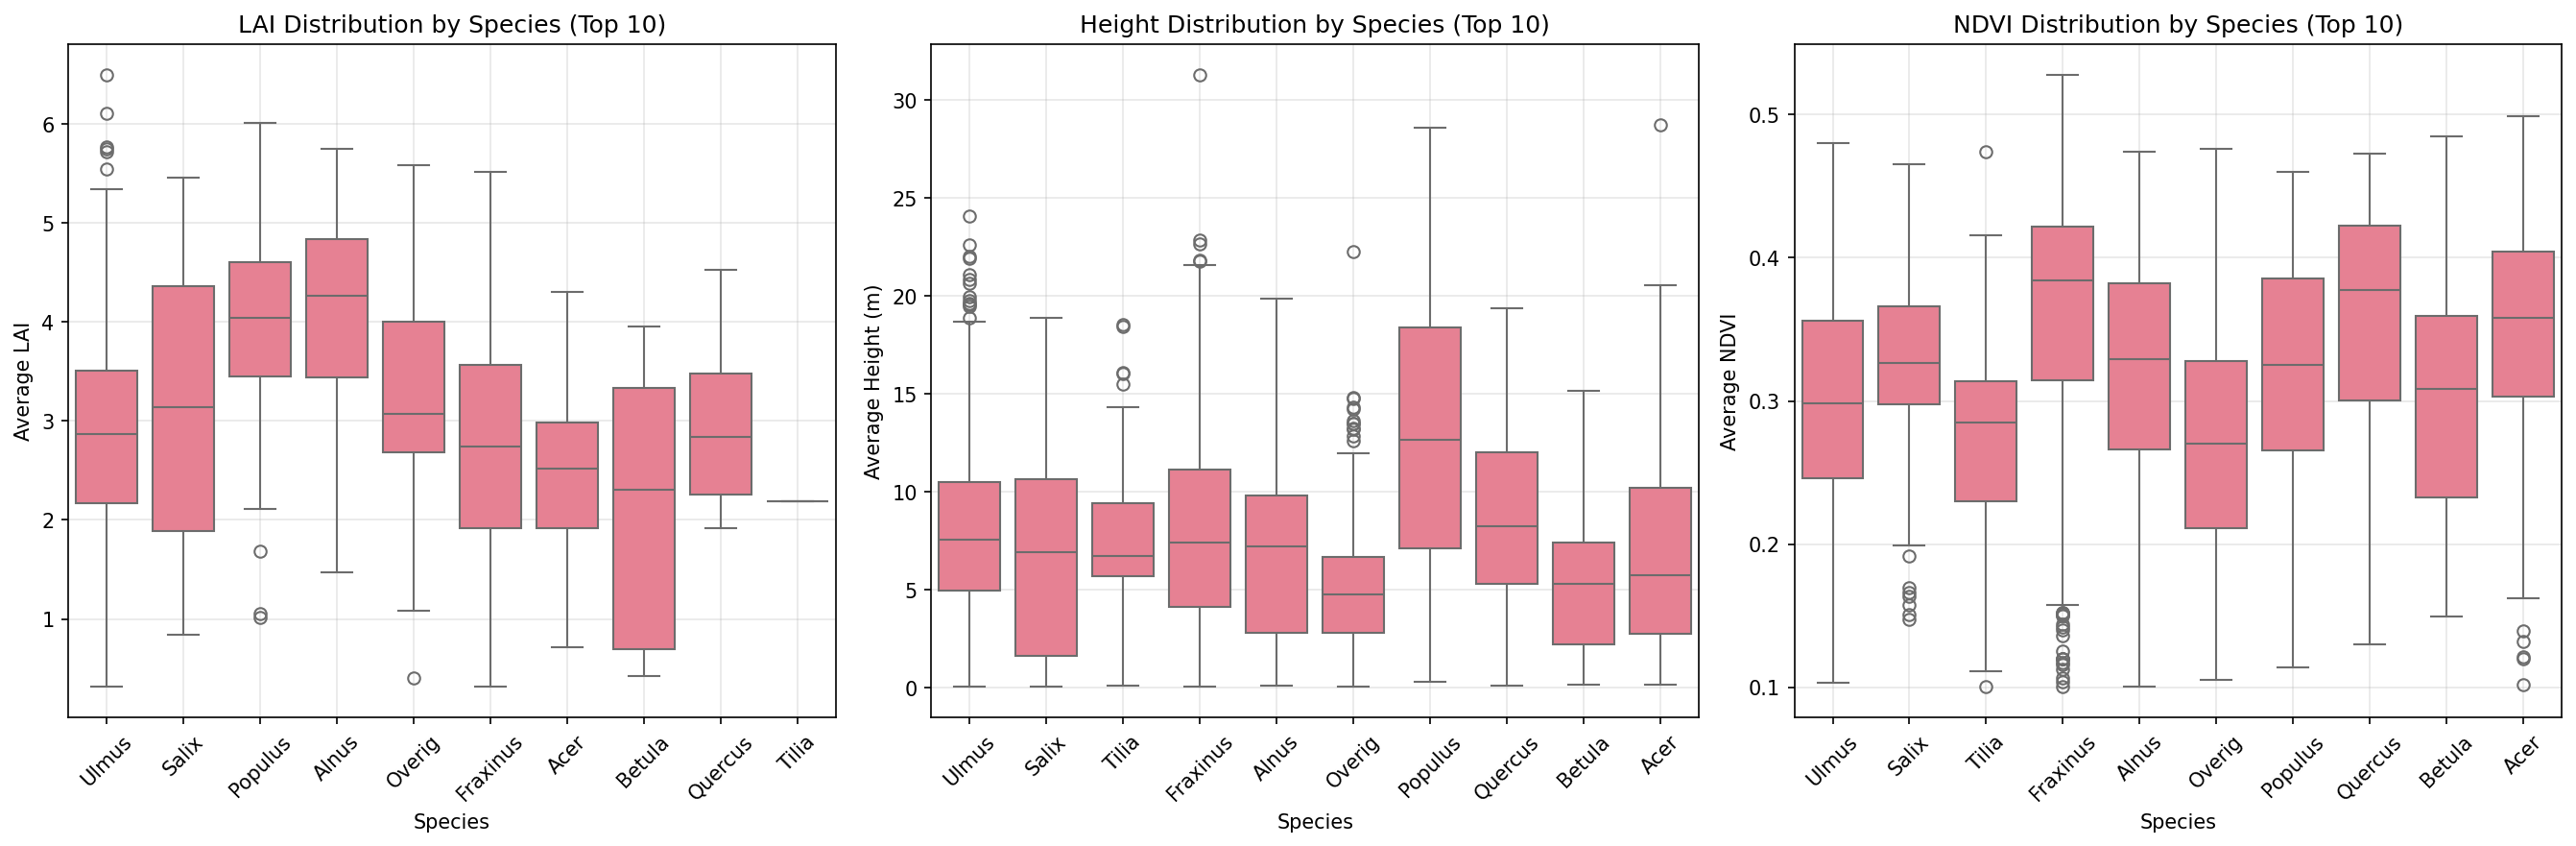
\includegraphics[width=\textwidth, height=\textheight, keepaspectratio]{figures/results/analytics/distributions_by_species.png}
    \caption{\textbf{Distribution of morphological and spectral features by tree species.} Multi-panel visualization showing the distribution of tree height, NDVI, and LAI values separated by species in the Amsterdam urban forest dataset. The proportions between species align with previous research on urban tree characteristics. Height distributions reflect typical urban factors such as tree age and municipal pruning practices. The LAI values are consistent with urban canopy studies, where values are typically lower than natural forests due to management practices and environmental stressors. Species-specific patterns validate the ecological realism of our LAI estimation methodology.}
    \label{fig:supp_species_distribution}
\end{figure}

\clearpage
